\section{System Methodology}
\label{sec:method}
\begin{figure*}[t]
\centering
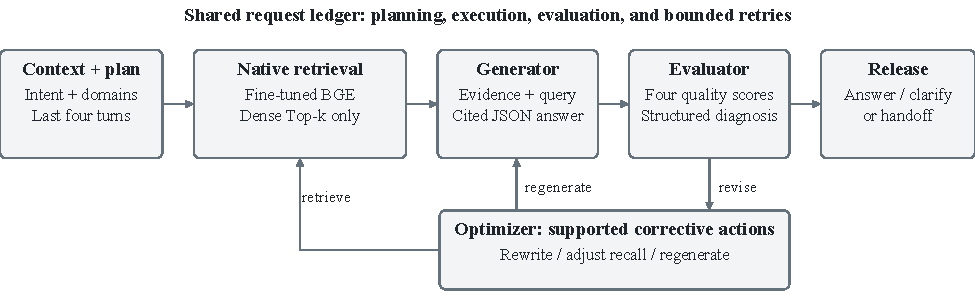
\includegraphics[width=\textwidth]{figures/architecture.pdf}
\caption{The selectable native fine-tuned configuration. Dense ranks are used directly without BM25, RRF, or Cross-Encoder reranking. Corrections are restricted to supported actions. Historical shared-model runs use the separate hybrid path; cross-domain continuation follows the branch-level protocol in Section~\ref{sec:setup}.}
\label{fig:architecture}
\end{figure*}

\subsection{Dialogue Planning}
The planner receives the current message and visible preceding turns. It returns a standalone query, intent, domain label, and optional subquestions. The domain is one of DMV, SSA, StudentAid, VA, or unknown. Unknown predictions may fall back to lexical cues in visible dialogue. The shared-model configuration allows at most three initial subquestions, normalizes whitespace, and removes duplicates. Gold domains, future turns, reference answers, and grounding labels remain outside online inputs.

The shared-model hybrid experiments use the standalone rewrite. For native fine-tuned retrieval, the initial query instead joins the last four visible user/agent turns with role labels and clears subqueries, matching retriever training. Domain prediction is advisory: global search is used unless a routing experiment explicitly applies predicted-domain filters. Gold metadata is not supplied to the planner.

% Integrated from retrievalreport_en.docx. Results are in 05_retrieval_existing.tex.
\subsection{Fine-Tuned and Hybrid Retrieval}
\label{sec:retrieval-method}
Two alternative paths share an evidence contract with stable document/passage IDs, source spans, and provenance. The current native fine-tuned preset selects struct passages and BGE checkpoint-2000, returning Dense cosine Top-10 directly. It disables BM25, RRF, Cross-Encoder reranking, subqueries, and additional semantic/per-document filtering. The retained hybrid path searches dense and lexical indexes in parallel, then fuses and optionally reranks candidates. These are alternatives, not consecutive stages of the fine-tuned path.

\paragraph{Structure-aware passages.}
Native index text joins the document title, ancestor titles, section title, and body. \emph{Section} groups spans by section ID and preserves standalone headings. \emph{Struct} merges adjacent spans sharing a section ID or stripped title, retaining a title path and coherent body. This keeps related policy sentences and conditions together, gives dense encoding a clearer subject, and lets BM25 match related terms within one passage. Fewer heading-only fragments compete for the final evidence slots. These are plausible mechanisms, rather than separately isolated effects.

\paragraph{Hybrid comparator and fusion.}
BGE-base-en-v1.5 uses 768-dimensional normalized CLS embeddings, a 512-token limit, its retrieval query prefix, and FAISS exact inner-product search. BM25 indexes the same passage text and removes user/agent query labels. Dense matching captures semantic similarity, while BM25 preserves exact service terms and form numbers. For the native hybrid study, Dense Top-100 and BM25 Top-50 are deduplicated and combined as
\begin{equation}
 \mathrm{RRF}(p)=\sum_{r:p\in L_r}
 \frac{1}{30+\mathrm{rank}_{L_r}(p)},
\end{equation}
where $L_r$ is a branch's ranked list. Fusion retains 50 candidates without comparing the branches' raw score scales.

\paragraph{Optional hybrid reranking.}
In the hybrid comparator, the MiniLM-L6-v2 MS MARCO Cross-Encoder jointly scores query--passage pairs. Its query places the current user question before earlier user questions. Short confirmations such as \emph{yes} keep RRF order because their meaning depends on the preceding agent turn. Pairwise inference adds query cost as candidate count and traffic grow. The fine-tuned path neither loads nor calls this model.

\paragraph{Dense adaptation.}
We also investigate replacing query-time reranking with an adapted Dense retriever. Training uses 20,607 deduplicated struct inputs and all 109.5M BGE parameters: AdamW, learning rate $2\!\times\!10^{-5}$, weight decay .01, batch size 8, 2,000 steps, gradient clipping at 1.0, warmup/decay, and seed 20261108. A scale-20 multi-positive contrastive loss rewards any labeled positive and masks unlabeled same-document negatives. Checkpoint 2000 is selected on dev160 (Hit@10 78.75, versus 77.50 at step 1000); document vectors are rebuilt for it. Adapted Dense directly ranks passages without BM25, RRF, or a Cross-Encoder. Section~\ref{sec:retrieval-study} compares the four native configurations.

\subsection{Cited Response Generation}
The generator receives the original request, standalone query, visible history, and retrieved evidence. The prompt exposes local aliases such as E1 and E2 and requests a JSON answer, citation list, and status. Aliases are mapped back to stable source IDs. An answered response must cite at least one supplied passage; an insufficient-evidence response must have no citations. Unknown citations and inconsistent recognized inline markers are rejected. One additional format-correction call is allowed using the same evidence and budget. These checks validate output structure and citation membership, rather than entailment.

\subsection{Evaluation and Action Selection}
The evaluator scores relevance, answer sufficiency, groundedness, and dialogue consistency on a zero-to-one scale. The respective thresholds are 0.7, 0.7, 0.8, and 0.8. A separate evidence-sufficiency field asks whether the current context could support a complete revision. This distinction prevents an answer omission from automatically being diagnosed as a retrieval failure.

Feedback specifies missing information, failure categories, suggested queries, and a proposed decision. Structured diagnoses take priority: misunderstanding suggests query rewriting, retrieval coverage suggests recall adjustment, ranking suggests reranking where supported, and answer defects suggest regeneration. The native fine-tuned path exposes no reranking capability; unsupported actions cannot silently enable a Cross-Encoder. Explicitly insufficient evidence redirects regeneration toward retrieval. Negative diagnoses, low scores, invalid citations, or non-answer status block approval. Missing user information may trigger clarification.

\subsection{Budgets and Stopping}
The application creates one ledger before planning and retains it throughout initial retrieval, generation, evaluation, and optimization. The real-model configuration allows 30,000 total tokens, 180 seconds, and two optimization retries, with a maximum of 1,024 output tokens per call. Before a call, the ledger reserves a conservative allowance; afterward it charges reported usage, including usage from rejected malformed responses. Unknown usage remains unavailable rather than becoming zero.

The controller stops on approval, clarification, escalation, a resource limit, unsupported actions, ineffective changes, or repeated unchanged state. Reusing adequate evidence for revision avoids unnecessary recall. An unchanged retrieval context normally stops the loop unless the diagnosis justifies answer revision. The retry bound counts optimization actions, not all model calls: format correction and separate evaluation calls also consume resources. Escalation prepares the dialogue, evidence, feedback, and attempted actions for handoff; the implementation does not deliver that package to a live human-service platform.
